\chapter{Semi-parametric and non-parametric models}\label{chap11}

\section*{Solutions of Exercises}\label{sec11_1}
\begin{enumerate}[leftmargin=*]

\item Simulate a semi-parametric regression where  
\begin{align*}
	y_i &= 0.5x_{i1} - 1.2x_{i2} + \mu_i, \\
	p(\mu_i) &= 
	0.3 \phi(\mu_i \mid -0.5,0.5^2) + 0.7 \phi(\mu_i \mid 1,0.8^2).		
\end{align*}
Assume that $x_{i1}$ and $x_{i2}$ follow a standard normal distribution and that the sample size is 1,000. Perform inference in this model assuming that the number of components is unknown. Start with $H=5$ and use non-informative priors, setting $\alpha_{h0}=\delta_{h0}=0.01$, $\bm{\beta}_0=\bm{0}_2$, $\bm{B}_0=\bm{I}_2$, $\mu_{h0}=0$, $\sigma^2_{\mu 0}=10$, and $\bm{\alpha}_0=[1/H \ \dots \ 1/H]^{\top}$. Use 6,000 MCMC iterations, a burn-in period of 4,000, and a thinning parameter of 2. Compare the population parameters with the posterior estimates and plot the population density along with the posterior density estimate of $\bm{\mu}$ (the mean, and the 95\% credible interval).\\

\textbf{Answer}

We can see from the posterior estimates that three components disappear after the burn-in iterations. The 95\% credible intervals encompass the population values of all parameters, and the posterior density estimate closely matches the population density. See Figure \ref{figPMPDens}, where the black line represents the population density, the blue line denotes the posterior mean density estimate, and the shaded light blue area corresponds to the 95\% credible interval.
 
\begin{tcolorbox}[enhanced,width=4.67in,center upper,
	fontupper=\large\bfseries,drop shadow southwest,sharp corners]
	\textit{R code. Semi-parametric Gaussian mixture}
	\begin{VF}
		\begin{lstlisting}[language=R]
rm(list = ls()); set.seed(010101)
# Simulate data from a 2-component mixture model
n <- 1000
x1 <- rnorm(n); x2 <- rnorm(n)
B <- c(0.5, -1.2); X <- cbind(x1, x2)
z <- rbinom(n, 1, 0.3)  # Latent class indicator
mu <- ifelse(z == 0, rnorm(n, -0.5, 0.5), rnorm(n, 1, 0.8))
plot(density(mu))
y <- X%*%B + mu
# Hyperparameters
d0 <- 0.001; a0 <- 0.001
b0 <- rep(0, 2); B0 <- diag(2); B0i <- solve(B0)
mu0 <- 0; sig2mu0 <- 10
H <- 5; a0h <- rep(1/H, H)
# MCMC parameters
mcmc <- 2000
burnin <- 4000
tot <- mcmc + burnin
thin <- 2
# Gibbs sampling functions
PostSig2 <- function(Beta, muh, Xh, yh){
	Nh <- length(yh)
	an <- a0 + Nh
	dn <- d0 + t(yh - muh - Xh%*%Beta)%*%(yh - muh - Xh%*%Beta)
	sig2 <- invgamma::rinvgamma(1, shape = an/2, rate = dn/2)
	return(sig2)
}
PostBeta <- function(sig2, mu, X, y, Psi){
	XtX <- matrix(0, 2, 2)
	Xty <- matrix(0, 2, 1)
	Hs <- length(mu)
	for(h in 1:Hs){
		idh <- which(Psi == h)
		if(length(idh) == 1){
			Xh <- matrix(X[idh,], 1, 2)
			XtXh <- sig2[h]^(-1)*t(Xh)%*%Xh
			yh <- y[idh]
			Xtyh <- sig2[h]^(-1)*t(Xh)%*%(yh - mu[h])
		}else{
			Xh <- X[idh,]
			XtXh <- sig2[h]^(-1)*t(Xh)%*%Xh
			yh <- y[idh]
			Xtyh <- sig2[h]^(-1)*t(Xh)%*%(yh - mu[h])
		}
		XtX <- XtX + XtXh
		Xty <- Xty + Xtyh
	}
	Bn <- solve(B0i + XtX)
	bn <- Bn%*%(B0i%*%b0 + Xty)
	Beta <- MASS::mvrnorm(1, bn, Bn)
	return(Beta)
}
\end{lstlisting}
	\end{VF}
\end{tcolorbox} 

\begin{tcolorbox}[enhanced,width=4.67in,center upper,
	fontupper=\large\bfseries,drop shadow southwest,sharp corners]
	\textit{R code. Semi-parametric Gaussian mixture}
	\begin{VF}
		\begin{lstlisting}[language=R]
Postmu <- function(sig2h, Beta, Xh, yh){
	Nh <- length(yh)
	sig2mu <- (1/sig2mu0 + Nh/sig2h)^(-1)
	mun <- sig2mu*(mu0/sig2mu0 + sum((yh - Xh%*%Beta))/sig2h)
	mu <- rnorm(1, mun, sig2mu^0.5)
	return(mu)
}
PostBetas <- matrix(0, mcmc+burnin, 2)
PostPsi <- matrix(0, mcmc+burnin, n)
PostSigma2 <- list(); PostMu <- list()
PostLambda <- list(); Reg <- lm(y ~ X)
Beta <- Reg$coefficients[2:3]; Res <- Reg$residuals
plot(density(Res))
Resq <- quantile(Res, c(0.2, 0.4, 0.6, 0.8))
Id1 <- which(Res <= Resq[1])
Id2 <- which(Res > Resq[1] & Res <= Resq[2])
Id3 <- which(Res > Resq[2] & Res <= Resq[3])
Id4 <- which(Res > Resq[3] & Res <= Resq[4])
Id5 <- which(Res > Resq[4])
Nh <- rep(n/H, H); Lambda <- rep(1/H, H)
MU <- c(mean(Res[Id1]), mean(Res[Id2]), mean(Res[Id3]), mean(Res[Id4]), mean(Res[Id5]))
Sig2 <- c(var(Res[Id1]), var(Res[Id2]), var(Res[Id3]), var(Res[Id4]), var(Res[Id5]))
Psi <- rep(NA, n); Hs <- length(MU)
pb <- winProgressBar(title = "progress bar", min = 0, max = tot, width = 300)
for(s in 1:tot){
	for(i in 1:n){
		lambdai <- NULL
		for(h in 1:Hs){
			lambdaih <- Lambda[h]*dnorm(y[i] - X[i,]%*%Beta, MU[h], Sig2[h]^0.5)
			lambdai <- c(lambdai, lambdaih)
		}
		Psi[i] <- sample(1:Hs, 1, prob = lambdai)
	}
	PostPsi[s, ] <- Psi
	Hs <- length(table(Psi))
	for(h in 1:Hs){
		idh <- which(Psi == h)
		Sig2[h] <- PostSig2(Beta = Beta, muh = MU[h], Xh = X[idh,], yh = y[idh])
		MU[h] <- Postmu(sig2h = Sig2[h], Beta = Beta, Xh = X[idh,], yh = y[idh])
	}
	PostSigma2[[s]] <- Sig2
	PostMu[[s]] <- MU 
	Beta <- PostBeta(sig2 = Sig2, mu = MU, X = X, y = y, Psi = Psi)
	PostBetas[s,] <- Beta
	Lambda <- sort(MCMCpack::rdirichlet(1, a0h[1:Hs] + table(Psi)), decreasing = TRUE)
	PostLambda[[s]] <- Lambda
	setWinProgressBar(pb, s, title=paste( round(s/tot*100, 0),"% done"))
}
close(pb)
\end{lstlisting}
	\end{VF}
\end{tcolorbox}

\begin{tcolorbox}[enhanced,width=4.67in,center upper,
	fontupper=\large\bfseries,drop shadow southwest,sharp corners]
	\textit{R code. Semi-parametric Gaussian mixture}
	\begin{VF}
		\begin{lstlisting}[language=R]
keep <- seq(burnin, tot, thin)
PosteriorBetas <- coda::mcmc(PostBetas[keep,])
summary(PosteriorBetas); plot(PosteriorBetas)
PosteriorPsi <- PostPsi[keep,]
Clusters <- sapply(1:length(keep), function(i){length(table(PosteriorPsi[i,]))})
PosteriorSIGMA <- matrix(NA, length(keep), 2)
PosteriorMU <- matrix(NA, length(keep), 2)
PosteriorLAMBDA <- matrix(NA, length(keep), 2)
l <- 1
for (s in keep){
	PosteriorSIGMA[l,] <- PostSigma2[[s]][1:2]
	PosteriorMU[l,] <- PostMu[[s]][1:2]
	PosteriorLAMBDA[l,] <- PostLambda[[s]][1:2]
	l <- l + 1
}
summary(coda::mcmc(PosteriorSIGMA))
summary(coda::mcmc(PosteriorMU))
summary(coda::mcmc(PosteriorLAMBDA))
# Posterior density estimate #
mus <- seq(-3, 4, 0.01)
DensityEst <- function(par, eval){
	lambda1 <- par[1]; lambda2 <- par[2]
	mu1 <- par[3]; mu2 <- par[4]
	sd1 <- par[5]; sd2 <- par[6]
	Dens <- lambda1 * dnorm(eval, mu1, sd1) + lambda2 * dnorm(eval, mu2, sd2)
	return(Dens)
}
par <- cbind(PosteriorLAMBDA, PosteriorMU, PosteriorSIGMA^0.5)
DensEval <- matrix(NA, length(keep), length(mus))
DensPop <- rep(NA, length(mus))
for(r in 1:length(mus)){
	for(l in 1:length(keep)){
		DensEval[l, r] <- DensityEst(par = par[l,], eval = mus[r])
	}
	DensPop[r] <- DensityEst(par = c(0.7, 0.3, -0.5, 1, 0.5, 0.8), eval = mus[r]) 
}
library(dplyr); library(ggplot2); require(latex2exp)
DataDens <- tibble(t = mus, Pop = DensPop, lower = apply(DensEval, 2, quantile, probs = 0.025), upper = apply(DensEval, 2, quantile, probs = 0.975), meanT = colMeans(DensEval))
plot_filtering_estimates <- function(df) {
	p <- ggplot(data = df, aes(x = t)) + 	geom_ribbon(aes(ymin = lower, ymax = upper), alpha = 1, fill = "lightblue") + 	geom_line(aes(y = Pop, color = "True Value"), linewidth = 0.5) + 	geom_line(aes(y = meanT, color = "Estimate"), linewidth = 0.5) +
	scale_color_manual(values = c("True Value" = "black", "Estimate" = "blue")) + xlab(TeX("$\\mu$")) + ylab("Density") + 	labs(title = "Density: Stochastic Errors", color = "") + theme_minimal()
	print(p)
}
plot_filtering_estimates(DataDens)
\end{lstlisting}
	\end{VF}
\end{tcolorbox}

\begin{figure}[!h]
	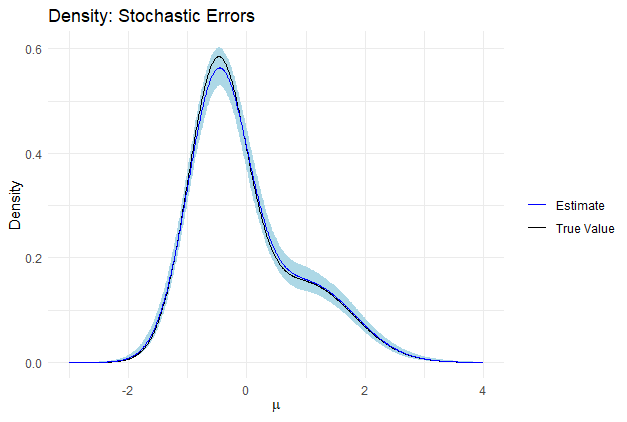
\includegraphics[width=340pt, height=200pt]{Chapters/chapter11/figures/DensEstSE.png}
	\caption[List of figure caption goes here]{Posterior density estimate: Stochastic errors.}\label{figPMPDens}
\end{figure}

\item Use the dataset \textit{MarijuanaColombia.csv} from our GitHub repository to perform inference on the demand for marijuana in Colombia. This dataset contains information on the (log) monthly demand in 2019 from the National Survey of the Consumption of Psychoactive Substances. It includes variables such as the presence of a drug dealer in the neighborhood (\textit{Dealer}), gender (\textit{Female}), indicators of good physical and mental health (\textit{PhysicalHealthGood} and \textit{MentalHealthGood}), age (\textit{Age} and \textit{Age2}), and (log) prices of marijuana, cocaine, and crack by individual (\textit{LogPriceMarijuana}, \textit{LogPriceCocaine}, and \textit{LogPriceCrack}). The sample size is 1,156.

Estimate a finite Gaussian mixture regression using non-informative priors, starting with five potential clusters. Obtain the posterior distribution of the own-price elasticity of marijuana and the cross-price elasticities of marijuana demand with respect to the prices of cocaine and crack.\\

\textbf{Answer:}

The following code demonstrates how to perform inference in this model using 2,000 MCMC iterations, with a burn-in period of 500 and a thinning parameter of 2. The results indicate the presence of two clusters, with mean probabilities of 0.73 and 0.27, and 95\% credible intervals of (0.66, 0.80) and (0.20, 0.34), respectively.  

The 95\% posterior credible intervals for the own-price elasticities are $(-0.69, -0.38)$ and $(-0.08, 0.30)$. Additionally, the 95\% credible intervals for the cross-price elasticities with respect to cocaine are $(0.12, 0.48)$ and $(-0.24, 0.18)$, while those with respect to crack are $(0.20, 0.60)$ and $(0.11, 0.50)$.  

These results suggest substitution between marijuana and both cocaine and crack: an increase in the prices of these drugs leads to higher marijuana demand, particularly in the first cluster of individuals. However, these findings should be interpreted with caution due to potential endogeneity issues that must be addressed for a rigorous scientific analysis. The primary goal of this exercise is pedagogical.  
 

\begin{tcolorbox}[enhanced,width=4.67in,center upper,
	fontupper=\large\bfseries,drop shadow southwest,sharp corners]
	\textit{R code. Semi-parametric Gaussian mixture}
	\begin{VF}
		\begin{lstlisting}[language=R]
rm(list = ls()); set.seed(010101)
Data <- read.csv("https://raw.githubusercontent.com/BEsmarter-consultancy/BSTApp/refs/heads/master/DataApp/MarijuanaColombia.csv")
attach(Data)
y <- LogMarijuana; X <- as.matrix(cbind(1, Data[,-1]))
Reg <- lm(y ~ X - 1); summary(Reg)
k <- dim(X)[2]; N <- dim(X)[1]
# Plot
library(ggplot2)
ggplot(Data, aes(x = LogMarijuana)) + geom_density(fill = "blue", alpha = 0.3) + labs(title = "Density Plot", x = "y", y = "Density") + theme_minimal()
# Hyperparameters
d0 <- 0.001; a0 <- 0.001
b0 <- rep(0, k); B0 <- diag(k); B0i <- solve(B0)
H <- 5; a0h <- rep(1/H, H)
# MCMC parameters
mcmc <- 2000; burnin <- 500
tot <- mcmc + burnin; thin <- 2
# Gibbs sampling functions
PostSig2 <- function(Betah, Xh, yh){
	Nh <- length(yh); an <- a0 + Nh
	dn <- d0 + t(yh - Xh%*%Betah)%*%(yh - Xh%*%Betah)
	sig2 <- invgamma::rinvgamma(1, shape = an/2, rate = dn/2)
	return(sig2)
}
PostBeta <- function(sig2h, Xh, yh){
	if(length(yh) == 1){
		Xh <- matrix(Xh, k, 1)
		Bn <- solve(B0i + sig2h^(-1)*Xh%*%t(Xh))
		bn <- Bn%*%(B0i%*%b0 + sig2h^(-1)*Xh%*%yh)
	}else{
		Bn <- solve(B0i + sig2h^(-1)*t(Xh)%*%Xh)
		bn <- Bn%*%(B0i%*%b0 + sig2h^(-1)*t(Xh)%*%yh)
	}
	Beta <- MASS::mvrnorm(1, bn, Bn)
	return(Beta)
}
PostBetas <- list(); PostSigma2 <- list(); PostLambda <- list()
PostPsi <- matrix(0, tot, N); Psi <- sample(1:H, N, replace = TRUE, prob = a0h)
Beta <- matrix(rep(Reg$coefficients, H), k, H); Hs <- H
\end{lstlisting}
	\end{VF}
\end{tcolorbox}

\begin{tcolorbox}[enhanced,width=4.67in,center upper,
	fontupper=\large\bfseries,drop shadow southwest,sharp corners]
	\textit{R code. Semi-parametric Gaussian mixture}
	\begin{VF}
		\begin{lstlisting}[language=R]
pb <- winProgressBar(title = "progress bar", min = 0, max = tot, width = 300)
for(s in 1:tot){
	Sig2 <- rep(NA, Hs)
	for(h in 1:Hs){
		idh <- which(Psi == h)
		Sig2[h] <- PostSig2(Betah = Beta[, h], Xh = X[idh,], yh = y[idh])
	}
	Hs <- length(Sig2)
	Beta <- matrix(NA, k, Hs)
	for(h in 1:Hs){
		idh <- which(Psi == h)
		Beta[, h] <- PostBeta(sig2h = Sig2[h], Xh = X[idh,], yh = y[idh])
	}
	Lambda <- sort(MCMCpack::rdirichlet(1, a0h[1:Hs] + table(Psi)), decreasing = TRUE)
	for(i in 1:N){
		lambdai <- NULL
		for(h in 1:Hs){
			idh <- which(Psi == h)
			lambdaih <- Lambda[h]*dnorm(y[i], X[i,]%*%Beta[,h], Sig2[h]^0.5)
			lambdai <- c(lambdai, lambdaih)
		}
		Psi[i] <- sample(1:Hs, 1, prob = lambdai)
	}
	Hs <- length(table(Psi))
	PostBetas[[s]] <- Beta; PostSigma2[[s]] <- Sig2
	PostLambda[[s]] <- Lambda; PostPsi[s, ] <- Psi
	setWinProgressBar(pb, s, title=paste( round(s/tot*100, 0),"% done"))
}
close(pb)
keep <- seq((burnin+1), tot, thin)
PosteriorPsi <- PostPsi[keep,]
Clusters <- sapply(1:length(keep), function(i){length(table(PosteriorPsi[i,]))})
NClus <- 2
# Clusters <- sapply(1:length(keep), function(i){print(table(PosteriorPsi[i,]))})
PosteriorSIGMA <- matrix(NA, length(keep), NClus)
PosteriorBETA <- array(NA, c(k,NClus,length(keep)))
PosteriorLAMBDA <- matrix(NA, length(keep), NClus)
l <- 1
for (s in keep){
	PosteriorSIGMA[l,] <- PostSigma2[[s]][1:NClus]
	PosteriorLAMBDA[l,] <- PostLambda[[s]][1:NClus]
	PosteriorBETA[,,l] <- PostBetas[[s]]
	l <- l + 1
}
summary(coda::mcmc(PosteriorSIGMA)); summary(coda::mcmc(PosteriorLAMBDA))
for(l in 1:NClus){
	PosteriorBeta <- t(PosteriorBETA[,l,])
	colnames(PosteriorBeta) <- c("Ct", names(Data[,-1]))
	print(summary(coda::mcmc(PosteriorBeta)))
}
\end{lstlisting}
	\end{VF}
\end{tcolorbox}

	\item Get the posterior sampler in the semi-parametric setting using a Dirichlet process mixture:
\begin{align*}
	y_i&=\boldsymbol{x}_i^{\top}\boldsymbol{\beta}+e_i\\
	e_i\mid \mu_i,\sigma_i^2 &\stackrel{iid}{\sim} N(\mu_i,\sigma_i^2),
\end{align*}
Do not include the intercept in $\boldsymbol{\beta}$ to get flexibility in the distribution of the stochastic errors.

\textbf{Answer:}

This mixture model can be expressed in a hierarchical structure:
\begin{align*}
	e_i\mid \boldsymbol{\theta}_i & \stackrel{ind}{\sim}f_{\boldsymbol{\theta}_i}\\
	\boldsymbol{\theta}_i \mid G & \stackrel{iid}{\sim} G\\
	G \mid \alpha,G_0 & \sim DP(\alpha G_0),
\end{align*}
where $e_i=y_i-\bm{x}_i^{\top}\bm{\beta}$. 

Thus, 

\begin{align*}
	s_i&\sim \sum_{h=0}^{\infty}\lambda_h\delta_h,\\
	e_i\mid s_i, \boldsymbol{\theta}_{s_i}&\sim N(\mu_{s_i},\sigma^2_{s_i}),
\end{align*} 
where $\lambda_h=P(\boldsymbol{\theta}_{i}=\boldsymbol{\theta}_{h}^*)$.

Let's assume $\boldsymbol{\beta}_i\mid \sigma^2_i\sim N(\boldsymbol{\beta}_0, \sigma^2_i\boldsymbol{B}_0)$, $\sigma_i^2\sim IG(\alpha_0/2,\delta_0/2)$, $\mu_i\sim N(\mu_0,\sigma_i^2/\beta_0)$, $\alpha\sim G(a,b)$ such that introducing the latent variable $\xi|\alpha,N\sim Be(\alpha+1,N)$, allows to easily sample the posterior draws of  $\alpha|\xi,H,\pi_{\xi}\sim\pi_{\xi}{G}(a+H,b-log(\xi))+(1-\pi_{\xi}){G}(a+H-1,b-log(\xi))$, where $\frac{\pi_{\xi}}{1-\pi_{\xi}}=\frac{a+H-1}{N(b-log(\xi))}$, $H$ is the number of atoms (mixture components). 

The conditional posterior distribution of $\boldsymbol\theta_i$ is
\begin{align*}
	\boldsymbol\theta_i|\left\{\boldsymbol\theta_{i'},\boldsymbol s_{i'}:i'\neq i\right\}, y_i, \alpha & \sim \sum_{i'\neq i}\frac{N_m^{(i)}}{\alpha+N-1}f_N(y_i|\boldsymbol{x}_i^{\top}\boldsymbol{\beta}_h,\sigma_h^2)\\
	& +\frac{\alpha}{\alpha+N-1}\int_{\mathcal{R}^K}\int_{0}^{\infty}f_N(y_i|\boldsymbol{x}_i^{\top}\boldsymbol{\beta},\sigma^2)f_N\left(\boldsymbol\beta\Big|\boldsymbol\beta_0,\sigma^2\boldsymbol B_0\right)f_{IG}(\sigma^2|\alpha_0,\delta_0)d\sigma^2 d\boldsymbol\beta,
\end{align*}
where $N_m^{(i)}$ is the number of observations such that $s_{i'}=h$, $i'\neq i$.

Observe that the probability of belonging to a particular cluster has a reinforcement property, as it increases with the cluster size; therefore, a DPM exhibits a self-reinforcing property, the more often a given value has been sampled in the past, the more likely it is to be sampled again.

Observe that the integral in the previous equation has exactly the same form as in the marginal likelihood presented in Section \ref{sec43}. Thus,
\begin{align*}
	p(y_i)&=\int_{\mathcal{R}^K}\int_{0}^{\infty}f_N(y_i|\boldsymbol{x}_i^{\top}\boldsymbol{\beta},\sigma^2)f_N\left(\boldsymbol\beta\Big|\boldsymbol\beta_0,\sigma^2\boldsymbol B_0\right)f_{IG}(\sigma^2|\alpha_0,\delta_0)d\sigma^2 d\boldsymbol\beta\\
	&=\frac{1}{\pi^{1/2}}\frac{\delta_0^{\alpha_0/2}}{\delta_n^{\alpha_n/2}}\frac{|{\boldsymbol{B}}_n|^{1/2}}{|{\boldsymbol{B}}_0|^{1/2}}\frac{\Gamma(\alpha_n/2)}{\Gamma(\alpha_0/2)}, 
\end{align*}
where $\alpha_n=1+\alpha_0$, $\delta_n=\delta_0 + y^{\top}y + \boldsymbol{\beta}_0^{\top}{\boldsymbol{B}}_0^{-1}\boldsymbol{\beta}_0 - \boldsymbol{\beta}_n^{\top}{\boldsymbol{B}}_n^{-1}\boldsymbol{\beta}_n$,  $\boldsymbol{B}_n = (\boldsymbol{B}_0^{-1} + \boldsymbol{x}\boldsymbol{x}^{\top})^{-1}$ and $\boldsymbol{\beta}_n = \boldsymbol{B}_n(\boldsymbol{B}_0^{-1}\boldsymbol{\beta}_0 + \boldsymbol{x}y)$.

Therefore, we sample $s_i$ as follows,
\begin{equation*}
	s_i|\left\{\boldsymbol\beta_{i'},\sigma_{i'}^2,\boldsymbol s_{i'}:i'\neq i\right\}, y_i, \alpha\sim\begin{Bmatrix}P(s_i=0|\cdot)=q_0^*\\
		P(s_i=h|\cdot)=q_h^*, h=1,2,\dots,H^{(i)}\end{Bmatrix},
\end{equation*}

where $H^{(i)}$ is the number of clusters excluding $i$, which may have its own cluster (singleton cluster), $q^*_c=\frac{q_c}{q_0+\sum_h q_h}$, $q_c=\left\{q_0,q_h\right\}$, $q_h=\frac{N_h^{(i)}}{\alpha+N-1}f_N(y_i|\boldsymbol{x}_i^{\top}\boldsymbol\beta_h,\sigma_h^2)$ and $q_0=\frac{\alpha}{\alpha+N-1}p(y_i)$.

If $s_i=0$ is sampled, then $s_i=H+1$, and a new $\sigma_h^2$ is sampled from $IG\left(\alpha_n/2,\delta_n/2\right)$, a new $\boldsymbol\beta_h$ is sample from $N(\boldsymbol\beta_n,\sigma_h^2\boldsymbol B_n)$.

Discarding $\boldsymbol\theta_h$'s from last step, we use $\boldsymbol s$ and total number of components to sample $\sigma_h^2$ from 

\begin{equation*}
	IG\left(\frac{\alpha_0+N_m}{2},\frac{\delta_0+\boldsymbol y_h^{\top}\boldsymbol y_h+\boldsymbol{\beta}_0^{\top}{\boldsymbol{B}}_0^{-1}\boldsymbol{\beta}_0-\boldsymbol{\beta}_{hn}^{\top}{\boldsymbol{B}}_{hn}^{-1}\boldsymbol{\beta}_{hn}}{2}\right),
\end{equation*}

where $\boldsymbol{B}_{hn}=(\boldsymbol{B}_0^{-1}+\boldsymbol{X}_h^{\top}\boldsymbol{X}_h)^{-1}$ and $\boldsymbol{\beta}_{hn}=\boldsymbol{B}_{hn}(\boldsymbol{B}_0^{-1}\boldsymbol{\beta}_0+\boldsymbol{X}_h^{\top}\boldsymbol{y}_h)$, $\boldsymbol{X}_h$ and $\boldsymbol{y}_h$ have the $\boldsymbol{x}_i$ and $y_i$ of individuals in component $h$. We sample $\boldsymbol\beta_h$ from
\begin{equation*}
	N\left({\boldsymbol\beta}_{hn},\sigma_h^2\boldsymbol B_{hn}\right),
\end{equation*}
$h=1,2,\dots,H$.


\item  Perform inference in the simulation of the semi-parametric model of Exercise 1 using the sampler of Exercise 3. 

 
\end{enumerate}